\documentclass[border=6pt]{standalone}
\usepackage{amsmath}
\usepackage{tikz}
\usetikzlibrary{arrows.meta}
\begin{document}
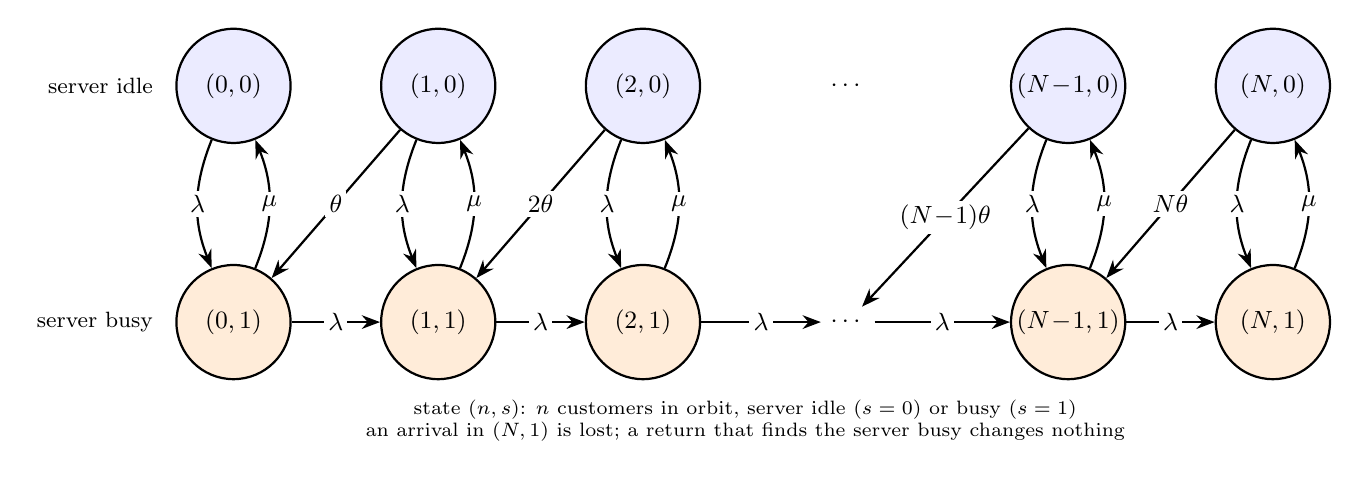
\begin{tikzpicture}[>=Stealth,font=\small,
 s/.style={draw,thick,circle,minimum size=1.1cm,inner sep=0pt,fill=blue!8},
 e/.style={->,thick},
 lab/.style={font=\small,fill=white,inner sep=1.5pt},
 every loop/.style={->,thick,looseness=6}]
\foreach \x/\n/\t in {0/0/0,2.6/1/1,5.2/2/2,10.6/Nm/N\!-\!1,13.2/N/N} {
  \node[s,minimum size=1.45cm] (i\n) at (\x,0) {$(\t,0)$};
  \node[s,minimum size=1.45cm,fill=orange!15] (b\n) at (\x,-3) {$(\t,1)$};
  \draw[e] (i\n) to[bend right=22] node[lab]{$\lambda$} (b\n);
  \draw[e] (b\n) to[bend right=22] node[lab]{$\mu$} (i\n);
}
\node (id) at (7.8,0) {$\cdots$};
\node (bd) at (7.8,-3) {$\cdots$};
\foreach \a/\b in {0/1,1/2,Nm/N} \draw[e] (b\a) -- node[lab]{$\lambda$} (b\b);
\draw[e] (b2) -- node[lab]{$\lambda$} (bd);
\draw[e] (bd) -- node[lab]{$\lambda$} (bNm);
\draw[e] (i1) -- node[lab,pos=0.5]{$\theta$} (b0);
\draw[e] (i2) -- node[lab,pos=0.5]{$2\theta$} (b1);
\draw[e] (iN) -- node[lab,pos=0.5]{$N\theta$} (bNm);
\draw[e] (iNm) -- node[lab,pos=0.5]{$(N\!-\!1)\theta$} (bd);
\node[font=\footnotesize,anchor=east] at (-0.9,0) {server idle};
\node[font=\footnotesize,anchor=east] at (-0.9,-3) {server busy};
\node[font=\scriptsize,align=center] at (6.5,-4.25) {state $(n,s)$: $n$ customers in orbit, server idle ($s=0$) or busy ($s=1$)\\an arrival in $(N,1)$ is lost; a return that finds the server busy changes nothing};
\end{tikzpicture}
\end{document}
